%%%%%%%%%%%%%%%%%%%%%%%%%%%%%%%%%%%%%%%%%%%%%%%%%%%%%%%%%%%%%%%%%%%%%%%%%%%%%%%%
\chapter{Обзор и сравнительный анализ существующих подходов}
%%%%%%%%%%%%%%%%%%%%%%%%%%%%%%%%%%%%%%%%%%%%%%%%%%%%%%%%%%%%%%%%%%%%%%%%%%%%%%%%
В данном разделе вводятся основные определения, связанные с предметной областью, приводятся различные классификации. Рассматриваются существующие подходы к обнаружению клонов и приводятся их основные характеристики.
%%%%%%%%%%%%%%%%%%%%%%%%%%%%%%%%%%%%%%%%%%%%%%%%%%%%%%%%%%%%%%%%%%%%%%%%%%%%%%%%
\section{Основные определения и классификация}

Для рассмотрения существующих подходов к обнаружению клонов, в первую очередь необходимо дать основные определения и классификации, связанные с предметной областью. 

\begin{itemize}
\setlength\itemsep{0mm}
\item \textbf{Фрагмент кода} - часть исходного кода, необходимая для запуска программы. Такая часть может содержать в себе функцию или метод, блоки или последовательности операторов.
\item \textbf{Клон кода} - две и более части кода, которые аналогичны друг другу в соответствии с типами клонов.
\item \textbf{Клоновый класс} - максимальное множество фрагментов кода, в котором любые два фрагмента являются клонами.
\item \textbf{Кандидат в клоны} - пара фрагментов кода, которые были определены как клон.
\end{itemize}

С точки зрения идентичности дублированных фрагментов, клоны делятся на следующие типы:
\begin{itemize}
\setlength\itemsep{0mm}
\item I: Полностью идентичные фрагменты программы без учета различий разметки и комментариев \cite{surveyroyandcordy} \cite{akhinitsykson}.
\item II: Клоны идентичные клонам первого типа, в которых также не учитваются различия идентификаторов, типов и литералов \cite{surveyroyandcordy} \cite{akhinitsykson}.
\item III: Клоны, идентичные клонам второго типа, в которых также не учитываются изменения, добавления и перемешивания операторов \cite{surveyroyandcordy} \cite{akhinitsykson}.
\item VI: Фрагменты программы, решающие схожую задачу, но реализованные различными способами (семантические клоны) \cite{surveyroyandcordy} \cite{akhinitsykson}.
\end{itemize}

При рассмотрении клонов с точки зрения их размера, выделяют следующие виды:
\begin{itemize}
\setlength\itemsep{0mm}
\item С фиксированной гранулярностью: идентичные фрагменты кода фиксированного размера (методы классы и т.д.).
\item С производной гранулярностью: идентичные фрагменты произвольного размера
\end{itemize}


%%%%%%%%%%%%%%%%%%%%%%%%%%%%%%%%%%%%%%%%%%%%%%%%%%%%%%%%%%%%%%%%%%%%%%%%%%%%%%%%


% \begin{figure}[htbp]
% \centering
% 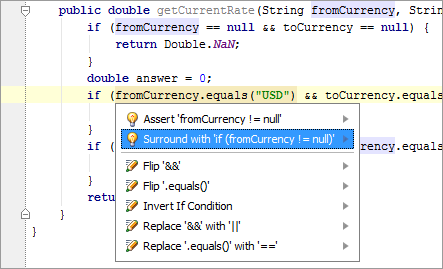
\includegraphics[width=\textwidth]{code_analysis_bugs.png}
% \caption{Рекомендации по проведению исследований в рамках диссертации}%
% \label{fig:how-to-do-research}
% \end{figure}
% 
% \Blindtext

%%%%%%%%%%%%%%%%%%%%%%%%%%%%%%%%%%%%%%%%%%%%%%%%%%%%%%%%%%%%%%%%%%%%%%%%%%%%%%%%
\section{Критерии сравнения}
%%%%%%%%%%%%%%%%%%%%%%%%%%%%%%%%%%%%%%%%%%%%%%%%%%%%%%%%%%%%%%%%%%%%%%%%%%%%%%%%

При анализе подходов к обнаружению дублированных участков необходимо выделить основные характеристики для их сравнения. 

%%%%%%%%%%%%%%%%%%%%%%%%%%%%%%%%%%%%%%%%%%%%%%%%%%%%%%%%%%%%%%%%%%%%%%%%%%%%%%%%
\section{Способы обнаружения клонов}
%%%%%%%%%%%%%%%%%%%%%%%%%%%%%%%%%%%%%%%%%%%%%%%%%%%%%%%%%%%%%%%%%%%%%%%%%%%%%%%%

Как правило, процесс обнаружения клонов состоит из двух этапов: трансформации и сравнения. На первом этапе код преобразуется в промежуточное внутреннее представление, которое позволяет использовать более эффективные и специализированные алгоритмы сравнения. В то же время, выбор промежуточного представления накладывает ограничения на используемые алгоритмы и во многом определяет качество итоговых результатов.

Методы поиска клонов могут быть классифицированы в зависимости от способа внутреннего представления кода:
\begin{itemize}
\setlength\itemsep{0mm}
\item на основе анализа текста
\item на основе анализа токенов
\item на основе анализа синтаксических деревьев
\item на основе анализа графов
\item на основе программных метрик
\item смешанные методы
\end{itemize}

\subsection{Метод основанный на анализе текста}

В 
% It is of great importance that you use correct references in your dissertation.
% Resent studies show that it can increase the chances of successful defense
% by as much as 3,17 percent~\cite{russian, java-book, ANTLR}.

